\documentclass{article}

\usepackage[utf8]{inputenc}
\usepackage{graphicx}
\usepackage{fancyhdr}
\usepackage{lastpage}
\usepackage{booktabs}
\usepackage{multirow}
\usepackage{array}
\usepackage[table]{xcolor}
\usepackage{scrextend}
\usepackage{enumitem}
\usepackage{hyperref}

\renewcommand*\rmdefault{iwona}
\renewcommand{\contentsname}{Indice}
\newcommand\tab[1][1cm]{\hspace*{#1}}\newcommand{\parnosep}[1]{\vspace*{-\baselineskip}\paragraph{#1}}
\newcommand{\subparnosep}[1]{\vspace*{-\baselineskip}\subparagraph{#1}}
\renewcommand{\labelenumii}{\theenumi\theenumii.}
\renewcommand{\theenumii}{.\arabic{enumii}}
\renewcommand{\labelenumiii}{\theenumi\theenumii\theenumiii.}
\renewcommand{\theenumiii}{.\arabic{enumiii}}
\newcommand{\nomeprogetto}[0]{B-Party}

\pagestyle{fancy}
\fancyhf{}
\rfoot{Pagina \thepage \hspace{1pt} di \pageref{LastPage}}

%Copertina e Indice
\title{\textbf{Prima Esercitazione\\Web Intelligence}}
\date{\today}
\author{\textit{Rosada Fabio} 851772\\}

\begin{document}
\pagenumbering{gobble}
\maketitle
\vfill
\newpage

\tableofcontents
\pagenumbering{arabic}

\section{Introduzione}
L'esercitazione è stata svolta su più file, per consentirne una più facile comprensione.
Per farla partire sarà sufficiente lanciare \textbf{main.py}, che a sua volta si occuperà di lanciare il resto.

Gli articoli sono salvati all'interno della cartella \textbf{articoli/} presente nella directory del progetto.

\section{Parte A}
La parte A è svolta nella sua interezza all'interno del file theverge\_downloader.py
\subsection{Generazione url archivio}
Per lo svolgimento della parte A dell'esercitazione, il sito scelto è stato www.theverge.com.\\Il sito offre una struttura ad archivio, quindi per prima cosa ho generato gli url delle pagine dell'archivio da cui successivamente recuperare i link degli articoli. Questa prima parte è stata abbastanza semplice in quanto per generare gli url è bastato aggiungere \textbf{/[categoria]/archives/[numero pagina]} allo url principale del sito.
\subsection{Recupero dei link degli articoli}Una volta fatto questo, aprendo le singole pagine tramite \textbf{urllib2} è bastato individurare la sezione contentente i link agli articoli tramite \textbf{BeautifulSoup} e recuperare il testo dei tag contententi l'attributo \textbf{href}. Una volta recuperati i link, li scrivo in un file, così se il download dei 1000 articoli dovesse essere interrotto, al prossimo avvio basterebe recuperare i link dal file senza "scansionare" nuovamente tutte le pagine dell'archivio.
\subsection{Salvataggio articoli}Analogamente, una volta recuperati i link dei 1000 articoli, tramite \textbf{BeautifulSoup} ho recuperato Titolo, Autore e Testo dell'articolo, e per ogni articolo ho creato un file che ha come prima riga il link dell'articolo, in modo da poterlo recuperare facilmente, come seconda riga il titolo, come terza l'autore e tutte le rimanenti sono dedicate al testo. Il nome del file è stato creato tramite la libreria \textbf{SHA} che mi consente di fare l'hash dello url, e di ottenere così un nome unico (per evitare sovrapposizioni).\\Durante quest'ultima fase però mi sono accorto che il sito in questione, per alcuni articoli utilizza una struttura completamente differente del corpo html, per semplicità quindi, nella prima fase della parte A, i link recuperati dell'archivio sono superiori a 1000 per assicurare almeno 1000 file scaricati nonostante gli errori.
\section{Parte B}
La parte B è stata volta all'interno del file analyzer.py, appoggiandosi a item\_reader.py per la lettura degli articoli (rirotna una lista contentente gli articoli già "puliti" dai caratteri che non ci interessano), e a gnuplot.py per la stampa dei grafici (in caso quest'ultima causare errori, in quanto utilizza gnuplot, basterà quindi commentarla).
\subsection{B.1 - analyzer.start\_base}
Questa parte consiste semplicemente nella creaione di un semplice dizionario delle occorrenze globali delle parole.
Una volta creato questo dizionario, salvo in una lista le parole presenti nel dizionario, ordinate per occorrenze.
In base a questa lista creo poi un file \textbf{.dat} utile per stampare poi il grafico tramite gnuplot.
Dirante questa fase ho selezionato poi alcune parole molto frequenti e di poca rilevanza, e le ho inserite poi nel file \textbf{stopwords.txt}
\begin{figure}[h]
	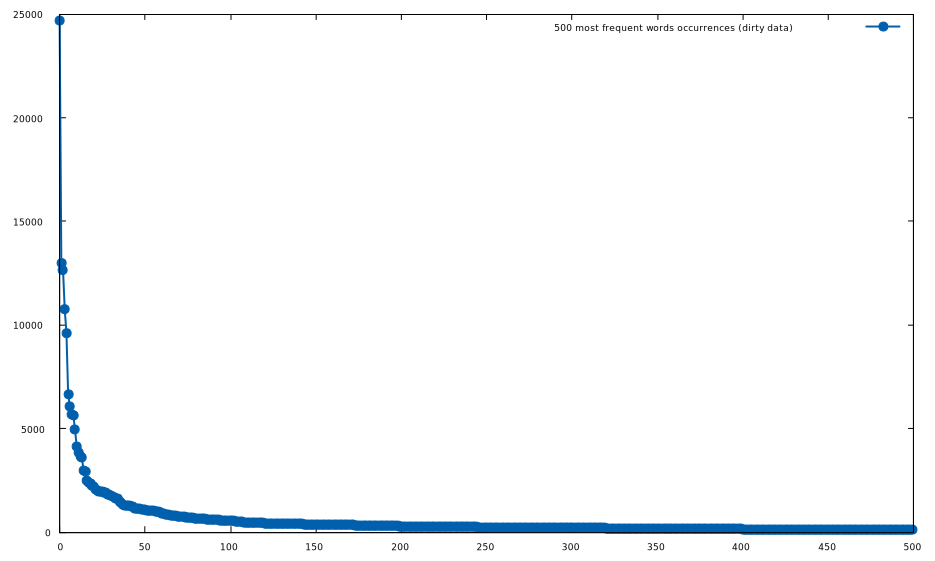
\includegraphics[width=9cm]{plotted_dirty.png}
	\centering
\end{figure}
\subsection{B.2 - analyzer.start\_advanced}
Similmente a come avviene nella parte B.1, in questa parte si andranno a contare le occorrenze e poi a creare il file \textbf{.dat} per stampare il grafico.
Questa volta però prima di contare le occorrenze, ci occuperemo di rimuovere le stopwords (leggendole dal file stopwords.txt), e tramite lemmatize trasformeremo le parole nei relativi lemmi (per esempio "he, she, it" vengono interpretati tutti come "he").
\begin{figure}[h]
	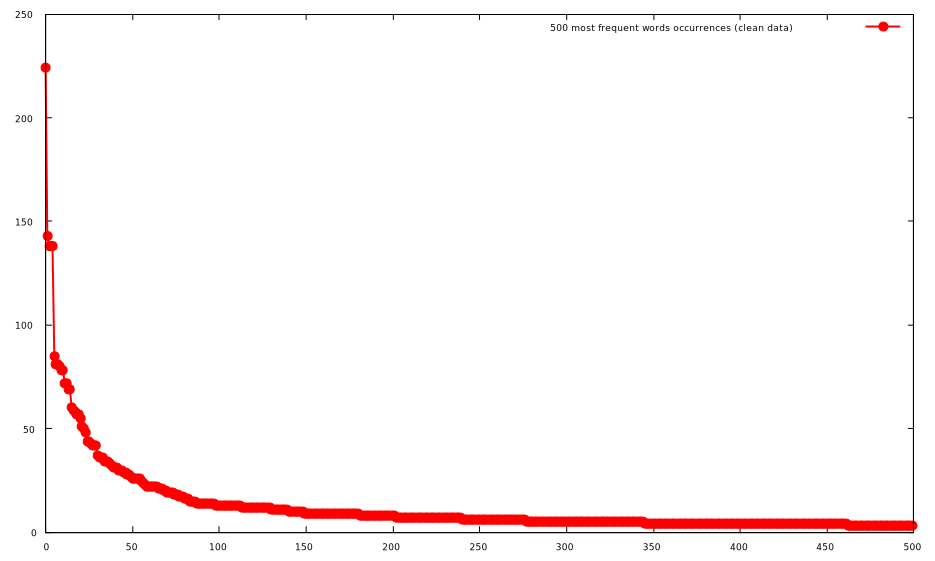
\includegraphics[width=10cm]{plotted_clean.png}
	\centering
\end{figure}
\newpage
\subsection{B.3 - analyzer.content\_recommender}
Questa parte utilizza in gran parte le librerie di \textbf{Gensim}, infatti per prima cosa creiamo un dizionario di tutte le parole presenti nei testi. Successivamente andremo a creare il corpus, ovvero una lista dove ogni elemento rappresenta un articolo, e questi elementi sono composti di una lista di tuple che rappresentano parola-occorrenze, tramite \textbf{tf-idf} andremo poi a dare un "peso" alle parole.

Dato che viene richiesto di dare i suggerimenti in base a N articoli, andremo ad inserire in corpus un nuovo articolo fittizio, che rappresenterà la "media" degli articoli scelti. Per fare ciò basta fare la media delle occorrenze nei vari articoli.

A questo punto non resta che creare la matrice di similarità (sempre tramite librerie di gensim) e in base a quella estrarre i suggerimenti.\\
\makebox[\textwidth]{\includegraphics[width=16cm]{content_recommender_base.png}}
\\I risultati possono essere considerati validi in quanto gli articoli suggeriti risultano essere simili a quelli più frequenti negli articoli di partenza, che come possiamo vedere, se pur con qualche eccezzione, risultano avere degli argomenti abbastanza omogenei.
\section{Parte C - analyzer.topic\_finder}
La parte C è molto simile alla parte b (infatti si basa sui dati creati in precedenza) con la differenza che modifica il corpus in base alla riduzione dimensionale (numero di topic) che scegliamo.
Una volta fatto questo, topic\_finder utilizza le stesse funzioni di supporto utilizzare da B.3 per trovare e stampare i suggerimenti.
Come prevedibile, per un numero molto basso di topic, e quindi per un numero molto basso di dimensioni, gli articoli tendono ad avere una somiglianza molto alta (in alcuni casi pari al 100\%), mentre per un numero molto alto (tendente al numero di articoli presenti) si tenderà ad avere un risultato simile a quello di partenza, in quanto la riduzione dimensionale sarà quasi inesistente.

\begin{figure}[h]
	\includegraphics[width=7.8cm]{k2.png}
	\centering
	\caption{con 1 solo topic gli articoli risultano essere tutti identici tra di loro}
\end{figure}
\begin{figure}[h]
	\includegraphics[width=7.8cm]{k950.png}
	\centering
	\caption{con 950 topic, gli articoli presentano una similarità molto simile a quella di partenza}
\end{figure}


\enddocument